% Options for packages loaded elsewhere
\PassOptionsToPackage{unicode}{hyperref}
\PassOptionsToPackage{hyphens}{url}
%
\documentclass[
]{article}
\usepackage{amsmath,amssymb}
\usepackage{lmodern}
\usepackage{ifxetex,ifluatex}
\ifnum 0\ifxetex 1\fi\ifluatex 1\fi=0 % if pdftex
  \usepackage[T1]{fontenc}
  \usepackage[utf8]{inputenc}
  \usepackage{textcomp} % provide euro and other symbols
\else % if luatex or xetex
  \usepackage{unicode-math}
  \defaultfontfeatures{Scale=MatchLowercase}
  \defaultfontfeatures[\rmfamily]{Ligatures=TeX,Scale=1}
\fi
% Use upquote if available, for straight quotes in verbatim environments
\IfFileExists{upquote.sty}{\usepackage{upquote}}{}
\IfFileExists{microtype.sty}{% use microtype if available
  \usepackage[]{microtype}
  \UseMicrotypeSet[protrusion]{basicmath} % disable protrusion for tt fonts
}{}
\makeatletter
\@ifundefined{KOMAClassName}{% if non-KOMA class
  \IfFileExists{parskip.sty}{%
    \usepackage{parskip}
  }{% else
    \setlength{\parindent}{0pt}
    \setlength{\parskip}{6pt plus 2pt minus 1pt}}
}{% if KOMA class
  \KOMAoptions{parskip=half}}
\makeatother
\usepackage{xcolor}
\IfFileExists{xurl.sty}{\usepackage{xurl}}{} % add URL line breaks if available
\IfFileExists{bookmark.sty}{\usepackage{bookmark}}{\usepackage{hyperref}}
\hypersetup{
  pdfauthor={Minuta de Índice de Relevância Econômica},
  hidelinks,
  pdfcreator={LaTeX via pandoc}}
\urlstyle{same} % disable monospaced font for URLs
\usepackage[margin=1in]{geometry}
\usepackage{graphicx}
\makeatletter
\def\maxwidth{\ifdim\Gin@nat@width>\linewidth\linewidth\else\Gin@nat@width\fi}
\def\maxheight{\ifdim\Gin@nat@height>\textheight\textheight\else\Gin@nat@height\fi}
\makeatother
% Scale images if necessary, so that they will not overflow the page
% margins by default, and it is still possible to overwrite the defaults
% using explicit options in \includegraphics[width, height, ...]{}
\setkeys{Gin}{width=\maxwidth,height=\maxheight,keepaspectratio}
% Set default figure placement to htbp
\makeatletter
\def\fps@figure{htbp}
\makeatother
\setlength{\emergencystretch}{3em} % prevent overfull lines
\providecommand{\tightlist}{%
  \setlength{\itemsep}{0pt}\setlength{\parskip}{0pt}}
\setcounter{secnumdepth}{-\maxdimen} % remove section numbering
\usepackage{booktabs}
\usepackage{longtable}
\usepackage{array}
\usepackage{multirow}
\usepackage{wrapfig}
\usepackage{float}
\usepackage{colortbl}
\usepackage{pdflscape}
\usepackage{tabu}
\usepackage{threeparttable}
\usepackage{threeparttablex}
\usepackage[normalem]{ulem}
\usepackage{makecell}
\usepackage{xcolor}
\ifluatex
  \usepackage{selnolig}  % disable illegal ligatures
\fi

\title{
\includegraphics[width=3in,height=\textheight]{logo-palacio.jpg}}
\author{Minuta de Índice de Relevância Econômica}
\date{Março de 2021}

\begin{document}
\maketitle

\renewcommand*\contentsname{Índice}
{
\setcounter{tocdepth}{2}
\tableofcontents
}
\newpage

\hypertarget{resumo}{%
\section{Resumo}\label{resumo}}

Foi feito primeiro estudo de relevância econômica de países a partir de
dados disponíveis publicamente relacionados a comércio, tecnologia,
investimentos e financiamento. A partir da padronização mais simples
possível, o estudo demonstra ser possível construir índice a partir da
união de diferentes bases de dados. É preciso ter cuidado, contudo, na
medida em que dados heterogêneos podem apresentar corte da realidade
problemático caso não sejam propriamente ponderados. A partir dos dados
apresentados, proponho:

\begin{enumerate}
\def\labelenumi{\arabic{enumi}.}
\tightlist
\item
  Avaliar a conveniência dos atuais dados utilizados;
\item
  Propor novos dados a serem incorporados ao estudo, inclusive critérios
  políticos;
\item
  Encontrar modelo adequado de ponderação dos diferentes indicadores
  envolvidos.
\end{enumerate}

\hypertarget{dados}{%
\section{Dados}\label{dados}}

\hypertarget{comuxe9rcio}{%
\subsection{Comércio}\label{comuxe9rcio}}

Dados de comércio, segundo o
\href{http://comexstat.mdic.gov.br/}{ComexStat} do Ministério da
Economia. Para fins deste estudo, optou-se por analisar a participação,
por país, no total das exportações e importações brasileiras.

\hypertarget{tecnologia}{%
\subsection{Tecnologia}\label{tecnologia}}

\hypertarget{patentes}{%
\subsubsection{Patentes}\label{patentes}}

Dados do INPI.

Os dados de patentes selecionados foram adquiridos no endereço
eletrônico do
\href{https://www.gov.br/inpi/pt-br/central-de-conteudo/estatisticas}{INPI,
setor de estatísticas}, setor de ``Indicadores de Propriedade
Intelectual''. Em breve análise, considerou-se que o indicador
\textbf{Depósito de patentes tipo Patentes de Invenção, por país de
origem} melhor representaria a participação estrangeira no conjunto de
depósitos de patentes no Brasil.

Segundo a Lei da Propriedade Industrial (Lei nº 9.279/96), tanto
patentes de invenção como modelos de utilidade são protegidos por
patentes. Os depósitos de patentes na modalidade de ``Patentes de
Invenção'' (PI) representam mais de 90\% dos pedidos de patentes no
Brasil. O próprio
\href{https://www.gov.br/inpi/pt-br/acesso-a-informacao/pasta-x/boletim-mensal/arquivos/documentos/indicadores-de-pi_2019.pdf}{relatório
do INPI} a respeito do assunto, ao analisar os pedidos de patentes
feitos por não residentes, trabalha com dados na modalidade de Patentes
de Invenção. Por essa razão, escolheu-se essa categoria no atual estudo.

As tabelas indicam a quantidade dos pedidos de patentes de 2000 até o
último ano disponível. No caso, o ano de 2019.

Para fins deste estudo, considerou-se que os dados de pedidos de patente
relativos ao último ano disponível pode apresentar oscilação nos dados -
a depender do ano, o número de patentes solicitado pode variar de acordo
com a conjuntura de curto prazo. Por isso, para evitar a variação,
optou-se pela soma de todos os pedidos de patente, por país, desde o
início da série temporal, no ano de 2000, até o ano de 2019.

\hypertarget{bolsistas-brasileiros-no-exterior}{%
\subsubsection{Bolsistas brasileiros no
exterior}\label{bolsistas-brasileiros-no-exterior}}

Dados da CAPES e do CNPQ entre os anos de 2017 e 2019.

Os dados do CNPQ foram coletados no
\href{http://dadosabertos.cnpq.br/pt_BR/dataset?q=bolsas}{portal dados
abertos} da própria instituição. Os dados diziam respeito a todas as
bolsas concedidas a estudantes de ensino superior no Brasil. Por isso,
os dados foram devidamente filtrados para que sejam analisados apenas as
bolsas de estudantes de doutorado no exterior.

O mesmo procedimento foi realizado em relação aos dados da CAPES. Os
dados da CAPES, contudo, foram organizados previamente pela própria
instituição, tambem em seu
\href{https://dadosabertos.capes.gov.br/organization/11b0c6b9-fe2e-4cb1-89a1-6e481a1c7b29?res_format=CSV\&groups=bolsas-ativas-em-programas-de-mobilidade-internacional\&organization=bolsas-e-auxilios}{portal
de dados abertos}, agregando apenas bolsas da modalidade internacional.

\hypertarget{outros-indicadores-possuxedveis}{%
\subsubsection{Outros indicadores
possíveis}\label{outros-indicadores-possuxedveis}}

Dados da OMPI.

O
\href{https://www.wipo.int/edocs/pubdocs/en/wipo_pub_gii_2020.pdf}{Relatório
anual Global Innovation Index 2020}, publicado pela OMPI, apresenta
índice escalonando o nível de inovação, por país. Este índice pode
eventualmente ser útil ao presente estudo.

\hypertarget{investimentos}{%
\subsection{Investimentos}\label{investimentos}}

\hypertarget{dados-de-estoque-por-controlador-final}{%
\subsubsection{Dados de Estoque, por controlador
final}\label{dados-de-estoque-por-controlador-final}}

\href{https://www.bcb.gov.br/content/estatisticas/Documents/Tabelas_especiais/TabelasCompletasPosicaoIDP.xlsx}{Dados
do Banco Central} a respeito da posição de investimento direto no País
(IDP)\footnote{De acordo com a nomenclatura BPM-6, adotada pelo Banco
  Central}. Optou-se pela discriminação do \textbf{estoque de
investimentos pelo critério do controlador final}, na medida em que
dados pelo critério do investidor imediato podem não representar
diretamente o país de origem da empresa controladora do investimento.

\hypertarget{outros-indicadores-possuxedveis-1}{%
\subsubsection{Outros indicadores
possíveis}\label{outros-indicadores-possuxedveis-1}}

\hypertarget{unctad---dados-de-estoque-de-investimentos-no-exterior}{%
\paragraph{UNCTAD - Dados de estoque de investimentos no
exterior}\label{unctad---dados-de-estoque-de-investimentos-no-exterior}}

Dados da UNCTAD. A UNCTAD oferece, em seu
\href{https://unctadstat.unctad.org/en/BulkDownload.html}{repositório de
dados}, dados de fluxos e estoques, internos e externos, de Investimento
Externo Direto. No
\href{https://unctadstat.unctad.org/7zip/US_FdiFlowsStock.csv.7z}{indicador
a respeito de investimentos}, é possível identificar a
\textbf{porcentagem de estoque de investimentos no exterior do país, em
relação ao estoque de investimentos mundiais}. Tal indicador pode ser
útil para o estudo, na medida em que interessa ao Brasil se aproximar e
manter diálogo com países com alto nível de estoque de investimentos no
exterior.

\hypertarget{ocde---dados-de-estoque-de-investimentos-de-pauxedses-da-ocde-no-brasil}{%
\paragraph{OCDE - Dados de estoque de investimentos de países da OCDE no
Brasil}\label{ocde---dados-de-estoque-de-investimentos-de-pauxedses-da-ocde-no-brasil}}

A base de dados da OCDE permite discriminar, segundo país destino, o
estoque de investimentos de cada um dos países membros da organização.
No entanto, este indicador estaria disponível apenas para os membros da
OCDE, excluindo países importantes, como China. Caso seja de interesse,
esses dados podem ser incorporados de maneira suplementar ao estudo.

\hypertarget{emprego}{%
\subsection{Emprego}\label{emprego}}

Não foram encontradas bases de dados a respeito de dados de emprego
associados a investimentos estrangeiros no Brasil. As
\href{https://www.bcb.gov.br/content/estatisticas/Documents/Tabelas_especiais/TabelasCompletasPosicaoIDP.xlsx}{tabelas
do Banco Central} apresentam o número de empregos criados por
investimentos estrangeiros, por unidade federativa, mas não apresenta
dados do país de origem dos investimentos. Como o Banco Central dispõe
de dados de emprego, faz sentido supor que a associação entre emprego e
investimentos, por país, seja viável. Talvez seja o caso de contato com
a divisão responsável pelo setor de estatísticas do Banco Central para
verificar a possibilidade de acesso a esses dados, caso eles existam.

\hypertarget{financiamento}{%
\subsection{Financiamento}\label{financiamento}}

\hypertarget{empruxe9stimos-diretos-de-longo-prazo---passivos}{%
\subsubsection{Empréstimos diretos de longo prazo -
passivos}\label{empruxe9stimos-diretos-de-longo-prazo---passivos}}

O
\href{https://www.bcb.gov.br/content/estatisticas/Documents/Tabelas_especiais/EmprestimosDiretosLongoPrazoPassivop.xls}{Banco
Central oferece dados}, discriminados por país, do fluxo de
``empréstimos diretos de longo prazo passivos'' associados à rubrica de
``Outros Investimentos'' da Conta Financeira do Balanço de Pagamentos.
No estudo, optou-se por selecionar o fluxo de empréstimos no último ano
disponível. Outras abordagens, como o acúmulo do fluxo de empréstimos ao
longo de um conjunto de anos, também podem ser aplicadas.

\hypertarget{outros-indicadores-possuxedveis-2}{%
\subsubsection{Outros indicadores
possíveis}\label{outros-indicadores-possuxedveis-2}}

\hypertarget{participauxe7uxe3o-estrangeira-no-capital-votante-de-instituuxe7uxf5es-do-sistema-financeiro-nacional}{%
\paragraph{Participação estrangeira no capital votante de instituções do
Sistema Financeiro
Nacional}\label{participauxe7uxe3o-estrangeira-no-capital-votante-de-instituuxe7uxf5es-do-sistema-financeiro-nacional}}

O
\href{https://www.bcb.gov.br/content/publicacoes/evolucaosfn/r202012/T4CE_Quadro\%2012\%20-\%20Participa\%C3\%A7\%C3\%A3o\%20estrangeira\%20no\%20capital\%20votante\%20de\%20institui\%C3\%A7\%C3\%B5es\%20do\%20SFN.pdf}{Banco
Central disponibiliza} o quantitativo de empresas do sistema financeiro
nacional controladas por capital estrangeiro. Apesar do BC não indicar o
tamanho de tais empresas, em termos de capital, tal informação pode
eventualmente ser útil caso incorporada ao estudo.

\hypertarget{endividamento-em-moeda-estrangeira}{%
\paragraph{Endividamento em moeda
estrangeira}\label{endividamento-em-moeda-estrangeira}}

O Banco Central também oferece, finalmente, a
\href{https://www.bcb.gov.br/content/estatisticas/Documents/Tabelas_especiais/DivMoeda_T.xlsx}{distribuição
por moeda da Dívida Externa brasileira}. Estes dados não são
discriminados por país, apenas por moeda, mas podem eventualmente
contribuir para o atual estudo.

\hypertarget{resultados}{%
\section{Resultados}\label{resultados}}

Como modelo meramente incipiente, optou-se pela construção do índice a
partir da participação, por país, de cada um dos indicadores
selecionados. Para permitir uma base comum de comparação, os dados
brutos foram transformados em porcentagem. Em vez de dados brutos de
comércio, porcentagem de exportações e importações. Em vez do número de
patentes, porcentagem das patentes depositadas no Brasil - e assim em
diante. Foram incorporados, segundo os mesmos critérios, dados de
investimentos; bolsistas de doutorado da CAPES e CNPQ no exterior; e
financiamento.

O resultado do estudo foi adquirido, portanto, da maneira mais simples
possível: o índice foi construiído a partir da soma de cada um desses
indicadores. O resultado bruto não parece satisfatório: em função de
suas participações nos indicadores de investimento e financiamento, as
Ilhas Cayman figuram entre os cinco países mais relevantes
economicamente para o Brasil. Ao excluir os paraísos fiscais, contudo,
Estados Unidos, China, França e Espanha ocupam as primeiras posições.
Chama atenção, no entanto, a ausência de qualquer país sul-americano
entre os 10 primeiros do índice. A Argentina, no cálculo preliminar,
ocupa apenas a 14ª posição.

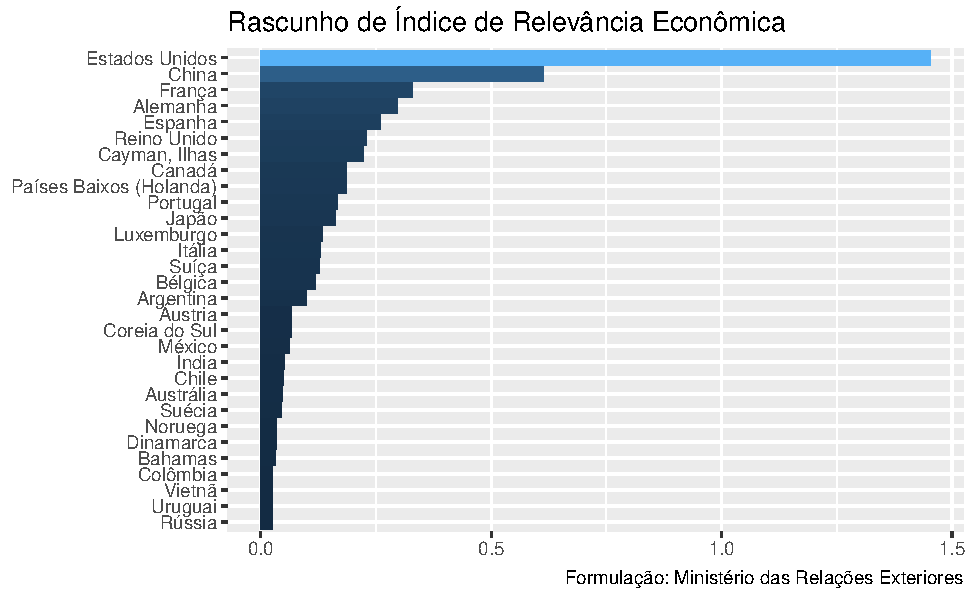
\includegraphics{relatório_files/figure-latex/unnamed-chunk-1-1.pdf}
\newpage \begingroup\fontsize{9}{11}\selectfont

\begin{longtable}[t]{>{\raggedleft\arraybackslash}p{5em}lr}
\toprule
\multicolumn{3}{c}{Índice de Relevância Econômica} \\
\cmidrule(l{3pt}r{3pt}){1-3}
Posição & País & Índice\\
\midrule
\endfirsthead
\multicolumn{3}{@{}l}{\textit{(continued)}}\\
\toprule
\multicolumn{3}{c}{Índice de Relevância Econômica} \\
\cmidrule(l{3pt}r{3pt}){1-3}
Posição & País & Índice\\
\midrule
\endhead

\endfoot
\bottomrule
\endlastfoot
\textbf{1} & Estados Unidos & 1.4526841\\
\textbf{2} & China & 0.6130139\\
\textbf{3} & França & 0.3300920\\
\textbf{4} & Alemanha & 0.2977868\\
\textbf{5} & Espanha & 0.2603531\\
\addlinespace
\textbf{6} & Reino Unido & 0.2292230\\
\textbf{7} & Cayman, Ilhas & 0.2225212\\
\textbf{8} & Canadá & 0.1870753\\
\textbf{9} & Países Baixos (Holanda) & 0.1860117\\
\textbf{10} & Portugal & 0.1656045\\
\addlinespace
\textbf{11} & Japão & 0.1622900\\
\textbf{12} & Luxemburgo & 0.1349852\\
\textbf{13} & Itália & 0.1301881\\
\textbf{14} & Suíça & 0.1266875\\
\textbf{15} & Bélgica & 0.1197706\\
\addlinespace
\textbf{16} & Argentina & 0.1003950\\
\textbf{17} & Áustria & 0.0671735\\
\textbf{18} & Coreia do Sul & 0.0669952\\
\textbf{19} & México & 0.0615383\\
\textbf{20} & Índia & 0.0524299\\
\addlinespace
\textbf{21} & Chile & 0.0492508\\
\textbf{22} & Austrália & 0.0477987\\
\textbf{23} & Suécia & 0.0445060\\
\textbf{24} & Noruega & 0.0351969\\
\textbf{25} & Dinamarca & 0.0336312\\
\addlinespace
\textbf{26} & Bahamas & 0.0311136\\
\textbf{27} & Colômbia & 0.0260327\\
\textbf{28} & Vietnã & 0.0252801\\
\textbf{29} & Uruguai & 0.0246878\\
\textbf{30} & Rússia & 0.0246370\\
\addlinespace
\textbf{31} & Singapura & 0.0225215\\
\textbf{32} & Malásia & 0.0221917\\
\textbf{33} & Paraguai & 0.0197956\\
\textbf{34} & Israel & 0.0197516\\
\textbf{35} & Indonésia & 0.0196090\\
\addlinespace
\textbf{36} & Taiwan (Formosa) & 0.0190535\\
\textbf{37} & Tailândia & 0.0188684\\
\textbf{38} & Finlândia & 0.0188333\\
\textbf{39} & Arábia Saudita & 0.0186015\\
\textbf{40} & Irlanda & 0.0185754\\
\addlinespace
\textbf{41} & Bermudas & 0.0169206\\
\textbf{42} & Turquia & 0.0166714\\
\textbf{43} & Emirados Árabes Unidos & 0.0160863\\
\textbf{44} & Hong Kong & 0.0156447\\
\textbf{45} & Peru & 0.0127235\\
\addlinespace
\textbf{46} & África do Sul & 0.0119855\\
\textbf{47} & Bolívia & 0.0116720\\
\textbf{48} & Argélia & 0.0104681\\
\textbf{49} & Marrocos & 0.0102092\\
\textbf{50} & Egito & 0.0096923\\*
\end{longtable}
\endgroup{}

\end{document}
